\label{arduino}

Der Arduino wurde 2005 von den beiden Entwicklern Massimo Banzi und David Cuartielles entwickelt. Der Mikrocomputer wurde nach einer Bar, in welcher sich die Entwickler gerne und oft trafen, benannt. Diese wiederum bekam ihren Namen nach Arduin von Ivrea, welcher von 1002 bis 1014 König von Italien war. \cite[vgl.]{Wikipedia.2020} \\
Aufgrund der hohen Anzahl von verschiedenen Arduino-Modellen, mussten wir uns darüber informieren, welches am besten für unser Projekt geeignet ist. Da wir uns selbst am Anfang des Projektes als Arduino-Einsteiger bezeichneten, wurde uns der in \ref{fig:ArduinoUno} zu sehende Arduino Uno empfohlen. Aufgrund von Rechercheergebnissen, dass dieses Modell das bekannteste und meist genutzte Arduino Board ist, entschieden wir uns dazu, dieses Modell zu nutzen. Diese Entscheidung hat den Hintergrund, dass uns so sehr viele Tutorials und Projektbeispiele im Internet zur Verfügung stehen. Diese sollen uns bei anfänglichem Erwerb von Grundwissen und späteren Projektproblemen weiterhelfen. \cite[vgl.]{GenerationROBOTS.26.09.2016} \\
Neben 13 digitalen und sechs analogen In- und Output-Pins besitzt der Arduino einen USB-B-Port, mit welchem das Laden eines neuen Programms ermöglicht wird. Die empfohlene Versorgungsspannung liegt beim Arduino Uno zwischen $7\volt$ und $12\volt$. \cite[vgl. S. 2]{sertronics.19.03.2020} Er besitzt, wie in \ref{fig:ArduinoUno} zu sehen, DC Pins von $5\volt$ und $3,3\volt$ DC-Spannung. \\
Speichermöglichkeiten gibt es auf dem Arduino zum Einen auf dem ATmega328, welcher eine Speicherkapazität von 32KB besitzt. Darauf werden allerdings 0,5KB vom Arduino Bootloader belegt. Zum Anderen verfügt er über 2KB SPRAM und 1KB EEPROM. \cite[vgl. S. 2]{sertronics.19.03.2020} Das ist auch der Grund dafür, weshalb die Daten später nicht auf dem Arduino selbst, sondern auf einer Mikro-SD-Karte gespeichert werden soll. Näheres dazu in Kapitel \ref{microSD}. \\

\begin{figure}[!hbt]
	\centering
	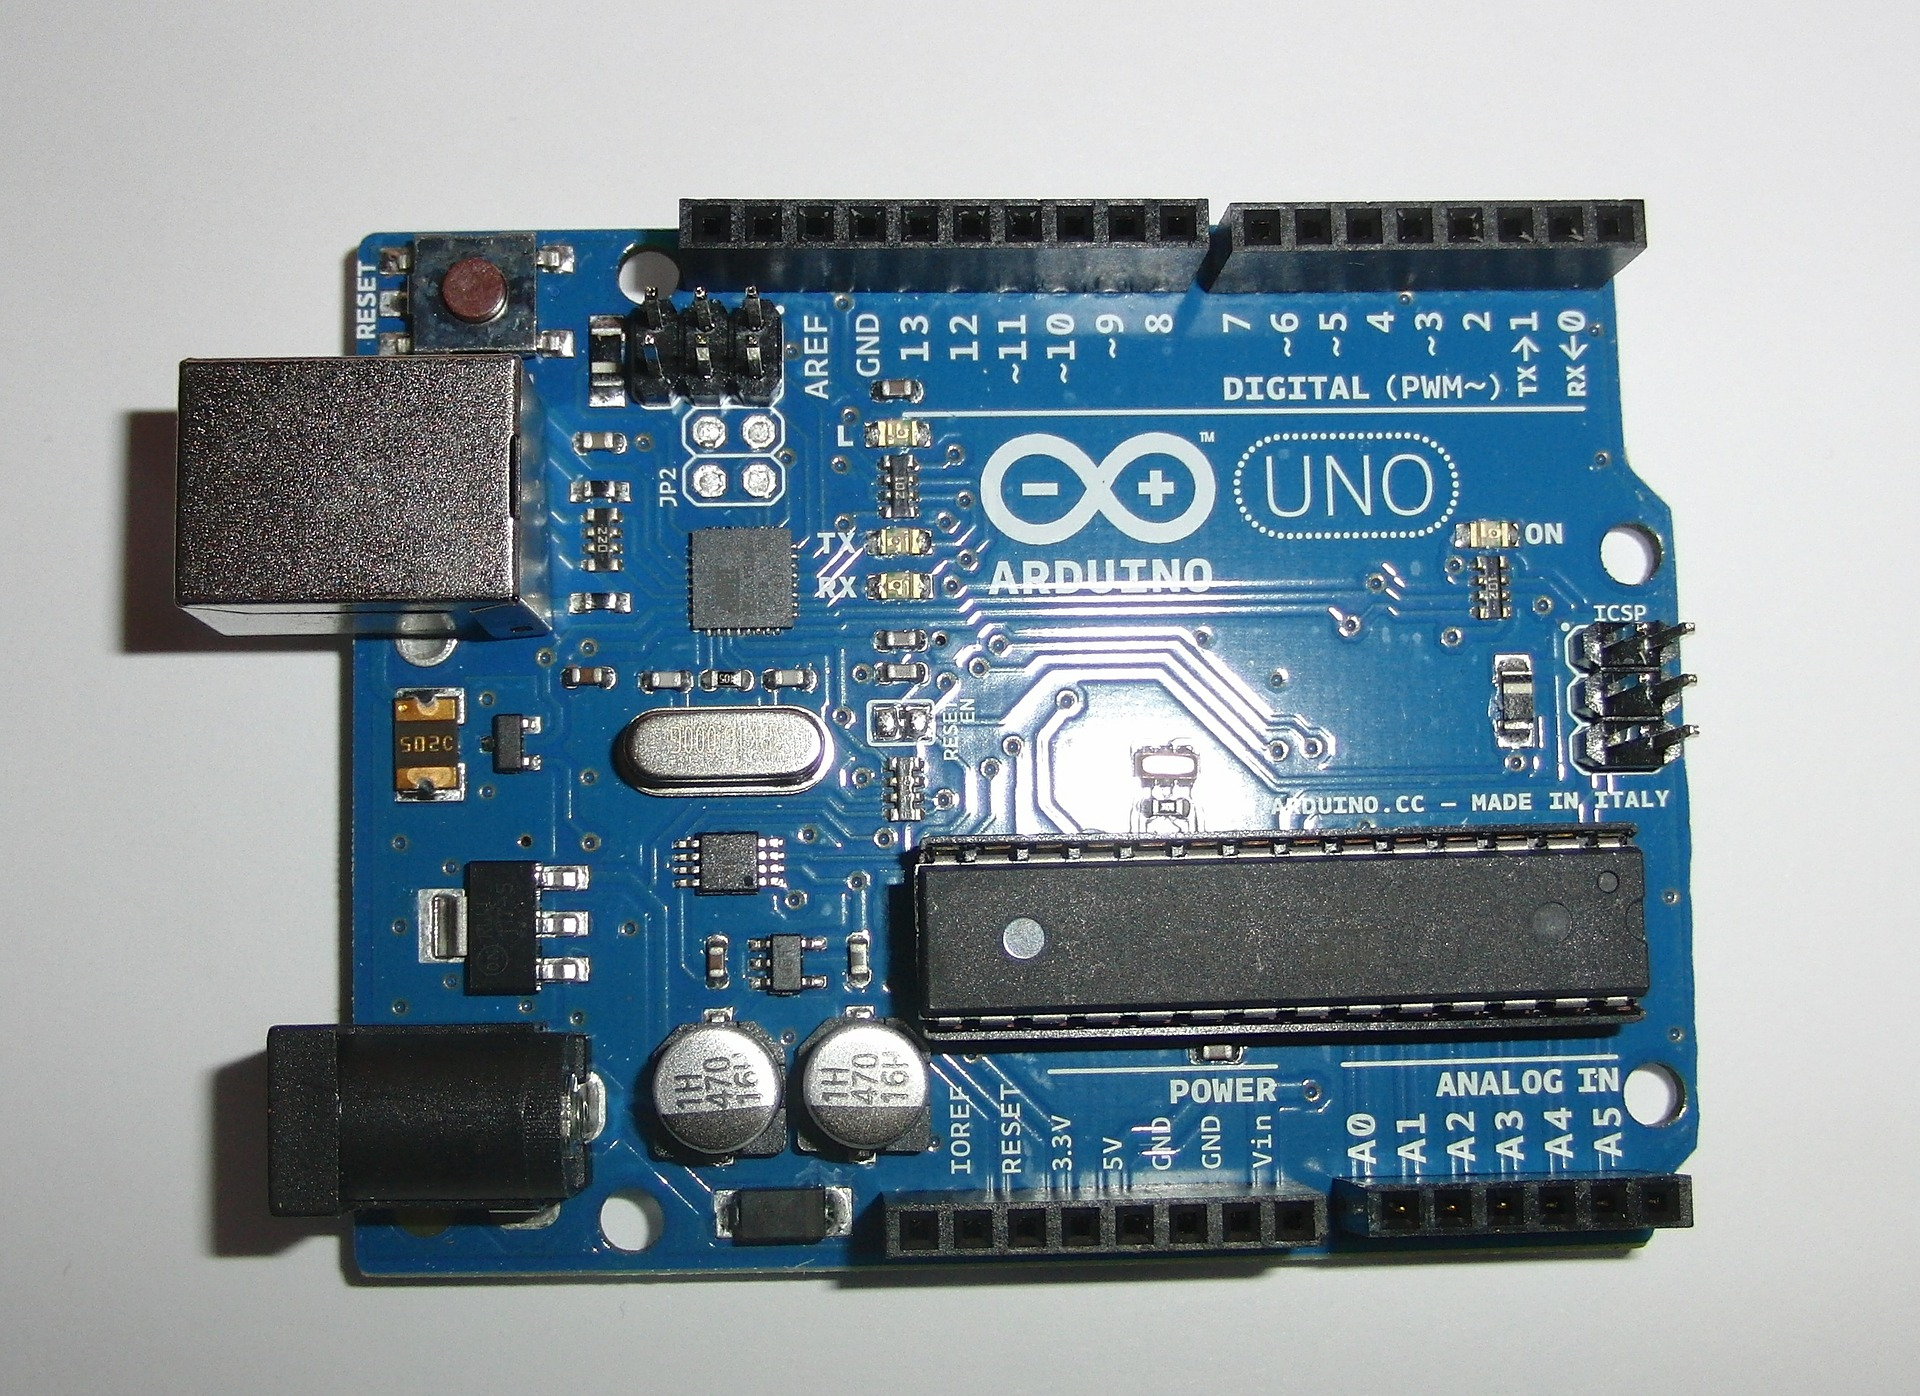
\includegraphics[width=0.6\linewidth]{Images/Arduino_Uno}
	\footnotesize \\Quelle: https://pixabay.com/de/photos/arduino-computer-cpu-373994/
	\caption{Arduino Uno}
	\label{fig:ArduinoUno}
\end{figure}
